%%%%%%%%%%%%%%%%%%%%%%%%%%%%%%%%%%%%%%%%%
% baposter Landscape Poster
% LaTeX Template
% Version 1.0 (11/06/13)
%
% baposter Class Created by:
% Brian Amberg (baposter@brian-amberg.de)
%
% This template has been downloaded from:
% http://www.LaTeXTemplates.com
%
% License:
% CC BY-NC-SA 3.0 (http://creativecommons.org/licenses/by-nc-sa/3.0/)
%
%%%%%%%%%%%%%%%%%%%%%%%%%%%%%%%%%%%%%%%%%

%----------------------------------------------------------------------------------------
%	PACKAGES AND OTHER DOCUMENT CONFIGURATIONS
%----------------------------------------------------------------------------------------

\documentclass[landscape,a0paper,fontscale=0.285]{baposter} % Adjust the font scale/size here

\usepackage{graphicx} % Required for including images
\graphicspath{{images/}} % Directory in which figures are stored

\usepackage{amsmath} % For typesetting math
\usepackage{amssymb} % Adds new symbols to be used in math mode
\usepackage{multirow}
\usepackage{booktabs} % Top and bottom rules for tables
\usepackage{enumitem} % Used to reduce itemize/enumerate spacing
\usepackage{palatino} % Use the Palatino font
\usepackage[font=small,labelfont=bf]{caption} % Required for specifying captions to tables and figures

\usepackage{multicol} % Required for multiple columns
\setlength{\columnsep}{1.5em} % Slightly increase the space between columns
\setlength{\columnseprule}{0mm} % No horizontal rule between columns

\usepackage{tikz} % Required for flow chart
\usetikzlibrary{shapes,arrows} % Tikz libraries required for the flow chart in the template

\newcommand{\compresslist}{ % Define a command to reduce spacing within itemize/enumerate environments, this is used right after \begin{itemize} or \begin{enumerate}
\setlength{\itemsep}{1pt}
\setlength{\parskip}{0pt}
\setlength{\parsep}{0pt}
}

\definecolor{lightblue}{rgb}{0.145,0.6666,1} % Defines the color used for content box headers

\begin{document}

\begin{poster}
{
headerborder=closed, % Adds a border around the header of content boxes
colspacing=2em, % Column spacing
bgColorOne=white, % Background color for the gradient on the left side of the poster
bgColorTwo=white, % Background color for the gradient on the right side of the poster
borderColor=gray, % Border color
headerColorOne=black, % Background color for the header in the content boxes (left side)
headerColorTwo=red, % Background color for the header in the content boxes (right side)
headerFontColor=white, % Text color for the header text in the content boxes
boxColorOne=white, % Background color of the content boxes
textborder=roundedleft, % Format of the border around content boxes, can be: none, bars, coils, triangles, rectangle, rounded, roundedsmall, roundedright or faded
eyecatcher=true, % Set to false for ignoring the left logo in the title and move the title left
headerheight=0.1\textheight, % Height of the header
headershape=roundedright, % Specify the rounded corner in the content box headers, can be: rectangle, small-rounded, roundedright, roundedleft or rounded
headerfont=\Large\bf\textsc, % Large, bold and sans serif font in the headers of content boxes
%textfont={\setlength{\parindent}{1.5em}}, % Uncomment for paragraph indentation
columns=5,
linewidth=2pt % Width of the border lines around content boxes
}
%----------------------------------------------------------------------------------------
%	TITLE SECTION 
%----------------------------------------------------------------------------------------
%
{}
%{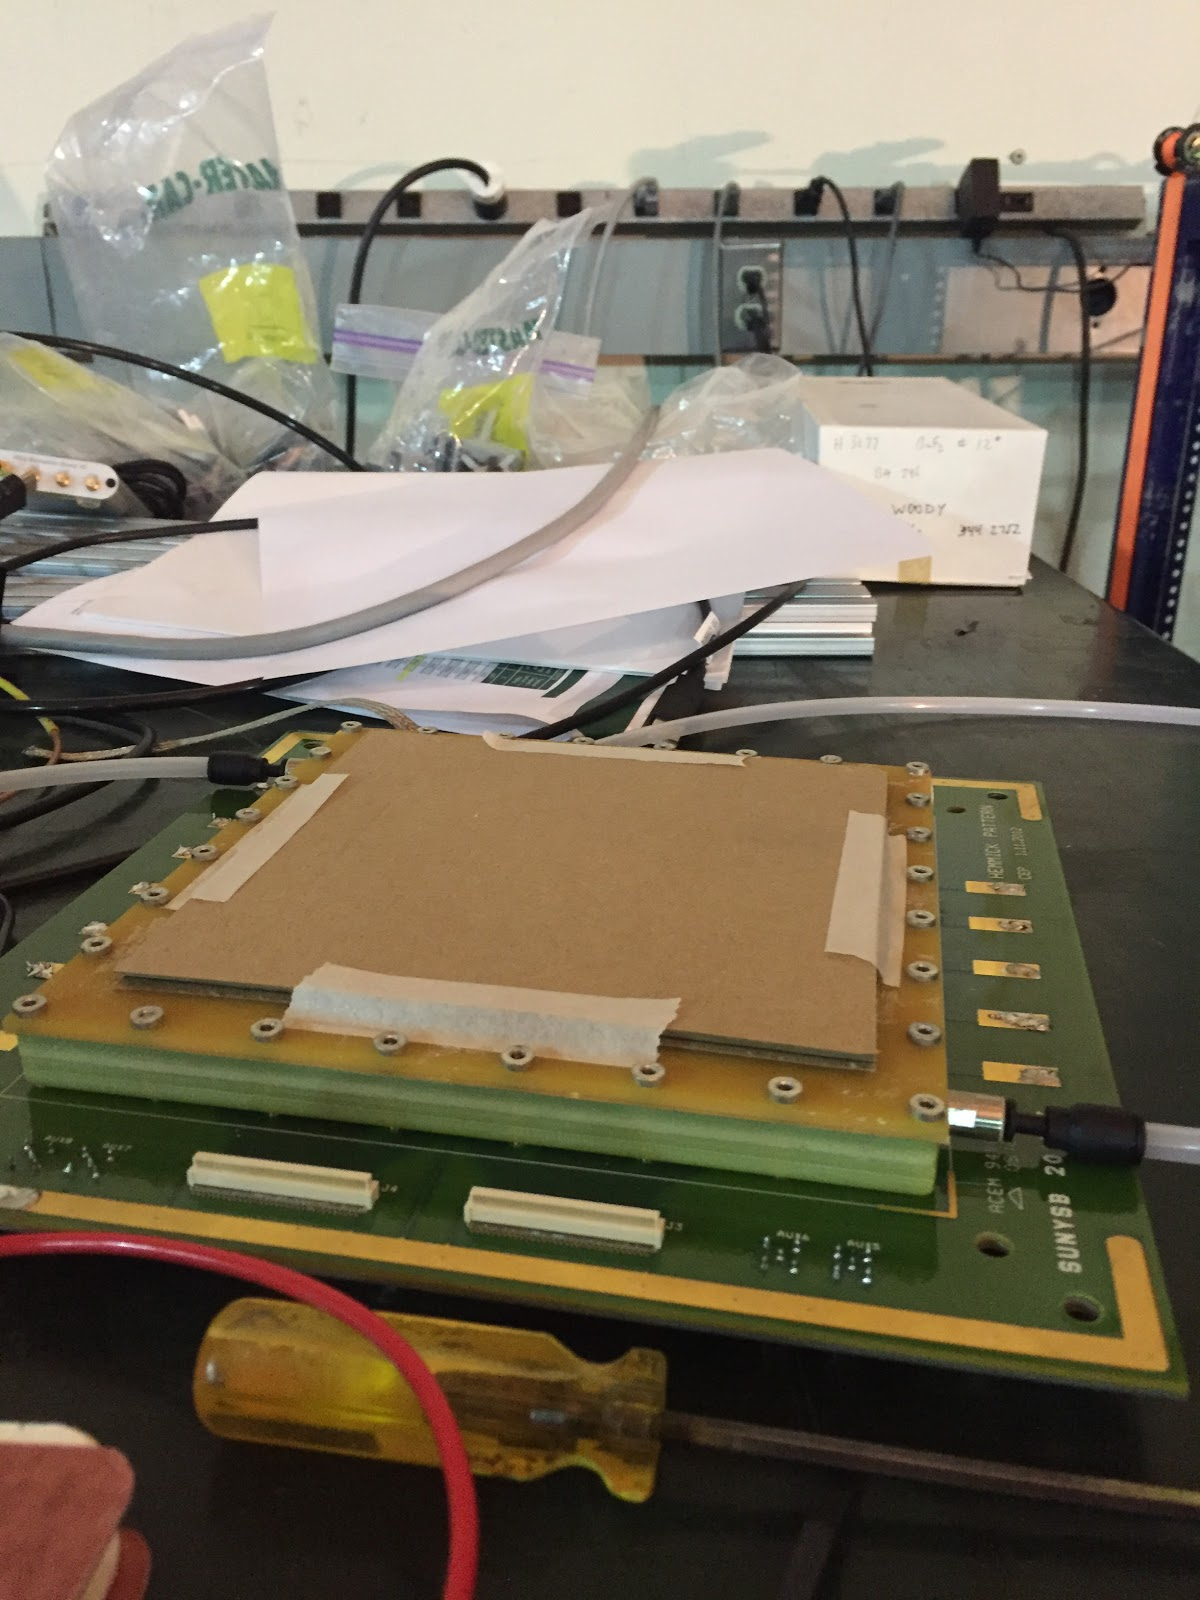
\includegraphics[height=4em]{Gem1.jpg}} % First university/lab logo on the left
{\bf\textsc{Unnecessarily Complicated Research Title}\vspace{0.5em}} % Poster title
{\textsc{\{ John Smith, James Smith and Jane Smith \} \hspace{12pt} University and Department Name}} % Author names and institution
%{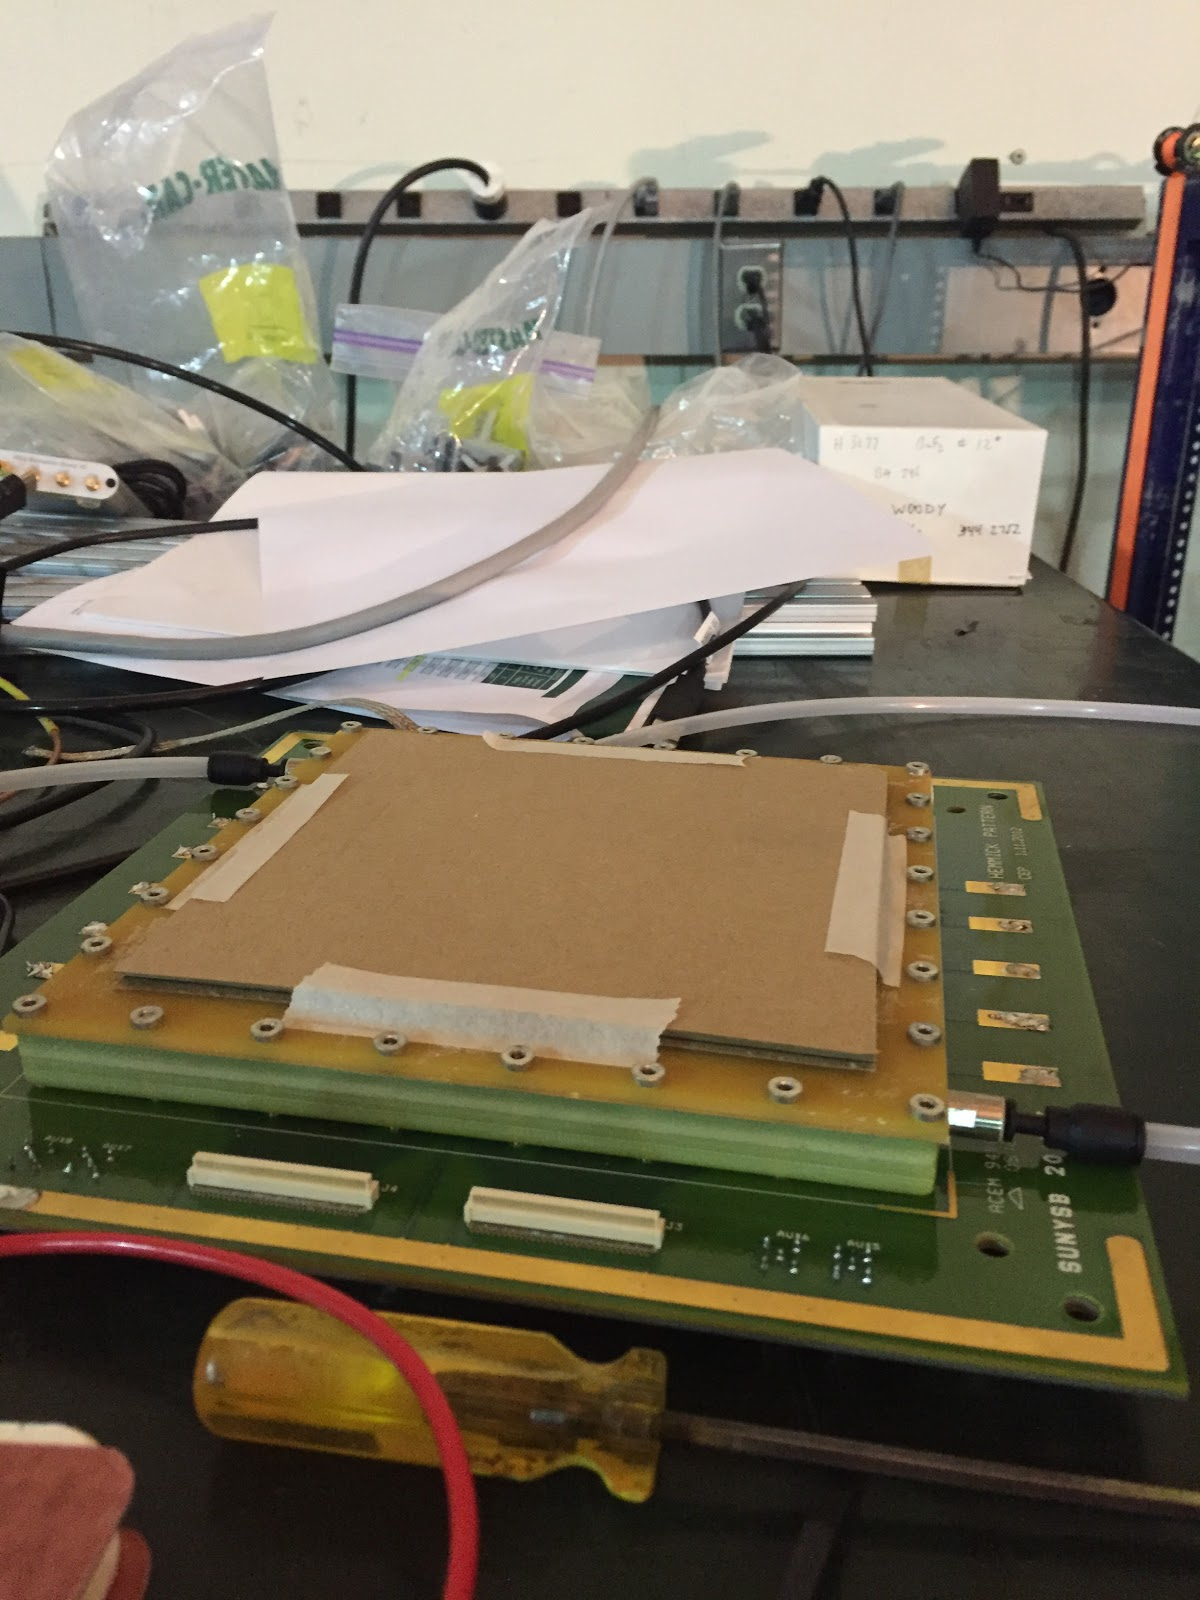
\includegraphics[height=4em]{Gem1.jpg}} % Second university/lab logo on the right
{}
%----------------------------------------------------------------------------------------
%	GEMS
%----------------------------------------------------------------------------------------

\headerbox{Gas Electron Multipliers (GEMs)}{name=gems,column=0,span=2,row=0}{
	\begin{paragraph}
		\indent Gas Electron Multipliers can be used to massively multiply an incoming flow of electrons for better detection. The GEMs we are using consist of a foil permeated by a high density of holes, which are stacked in layers of 1-3. Below the GEM foils lies a readout plane that is composed of a grid of wires responsible for recording the data associated with the incoming electrons. A voltage is applied to the foils but is broken up by a series of voltage dividers in such a way that each plate receives a fraction of the voltage. The voltage is distributed such that each successive plate has more voltage than the last so that in each gap between plates there exists an electric field. The magnitude of an electric field is dependent on potential difference, hence its existence stemming from the potential difference between each foil. This electric field is responsible for the multiplication of electrons as the initial current moves through the foils and subsequently through the generated electric field. \\
	\end{paragraph}
	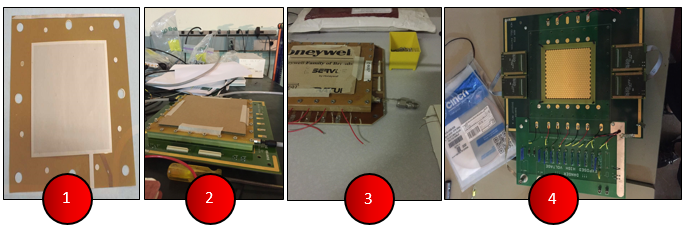
\includegraphics[width=12cm]{Gem4.png}\\
	\begin{paragraph}
		\indent Picture (1) is a sample of the GEM foils we are using. They are relatively paper thin, perforated with holes nearly too small to see with the human eye, and have a reflective surface. Pictures (5) and (6) display the readout plane and voltage dividers that are used along with the GEM foils. As seen in picture (5), the readout plane is a layout of wires connected in a geometric pattern; in this case they are arranged hexagonally. Pictures (3) and (4) are samples of the entire apparatus that includes the gas volume, GEM foil(s), readout plane and voltage dividers. The gas is distributed into the volume via the small device on the far right of picture (4), for example. Once the gas fills the volume, the particle can then be directed into the volume which will ionize the gas and the emitted electrons will flow through the GEM foil(s) and into the readout plane. For our setup we only expect to use 1-3 layers of the GEM foils. 
	\end{paragraph}
}

%----------------------------------------------------------------------------------------
%	ABSTRACT
%----------------------------------------------------------------------------------------

\headerbox{Abstract}{name=abstract,column=2,span=1,row=0}{
	\indent The Time Projection Chamber (TPC) of sPHENIX, the new experiment at RHIC / BNL, uses Gas Electron Multiplier (GEM) foils to amplify the ionization signals from charged particles passing through its gas volume. We have assembled a test setup using two GEM foils backed with readout planes inside a small gas volume. We present the status and progress in commissioning and testing the system with directly induced charges and an Iron-55 source.
	
	
}
%----------------------------------------------------------------------------------------
% FUTURE RESEARCH
%----------------------------------------------------------------------------------------

\headerbox{Future Research}{name=future,column=2,span=1,row=0,below=gems,above=bottom}{
	\vspace{5em}
}
%----------------------------------------------------------------------------------------
% DIAGRAMS
%----------------------------------------------------------------------------------------

\headerbox{Diagrams}{name=diagrams,column=2,span=1,row=0,below=abstract,above=future}{
	
}


%----------------------------------------------------------------------------------------
%	HARDWARE
%----------------------------------------------------------------------------------------

\headerbox{Hardware}{name=hardware,column=3,span=2,row=0}{	
\vspace{30em}
}

%----------------------------------------------------------------------------------------
%	SOFTWARE
%----------------------------------------------------------------------------------------

\headerbox{Software}{name=software,column=3,span=2,row=0,below=hardware,above=future}{	
}

%----------------------------------------------------------------------------------------
% CONCLUSION
%----------------------------------------------------------------------------------------

\headerbox{Conclusion}{name=conclusion,column=0,span=2,row=0,below=gems,above=bottom}{

}

%----------------------------------------------------------------------------------------
% REFERENCES
%----------------------------------------------------------------------------------------

\headerbox{References}{name=references,column=3,span=2,row=0,above=bottom,aligned=future}{
	
}



\end{poster}

\end{document}
